\section{Validity of the re-implemented estimators}
\label{app:e0}

All arms are run on a table of exact coalition values so that $10^5$ reruns remain affordable, which requires re-implementing the estimators. Before any result was produced we compared the re-implemented KernelSHAP at its shipped default with the library's own explainer on four settings: German Credit with an MLP ($d=20$), ACS Employment with an MLP and with gradient-boosted trees ($d=16$), and German Credit with logistic regression restricted to $d=10$, where the library enumerates all coalitions. Six instances were rerun 100 times per setting. In the three sampled settings the top-1 hit rates are identical, the top-3 and top-5 hit rates differ by at most 0.13 (binomial standard error of a difference at most 0.07), the per-attribute mean differs by at most 3.1 standard errors, and the ratio of rerun standard deviations lies between 0.96 and 1.04. In the enumerated setting both return the exact value to numerical precision. We read this as agreement of the two implementations in distribution, with the remaining per-attribute mean differences, up to 3.1 standard errors over many attributes, not separately explained.


\section{Additional results}
\label{app:extra}

\paragraph{Beyond $d=20$.}
A supplementary check on one further dataset (Arrhythmia, gradient-boosted trees on the margin scale, one seed, 20 instances) uses the interventional TreeSHAP value as the exact reference, so that $d$ is not limited by enumeration. At $d=40$ (a subset of the attributes) and $d=100$, the shipped KernelSHAP default returns the exact top-3 in a mean of $0.55$ and $0.49$ of the reruns at the shipped budget, and between $0.33$ and $0.58$ at every budget from a quarter to $16\times$ the shipped one. Paired \texttt{l1\_reg=False} reaches $0.98$--$1.00$ at the shipped budget and above, and Permutation with 500 evaluations $0.94$ and $0.96$. The $\ell_1$ truncation is therefore not specific to German Credit and does not vanish above $d=20$; with one model, one seed and 20 instances this checks that, and does not estimate how much of it a typical task shows.

\begin{figure}[h]
\centering
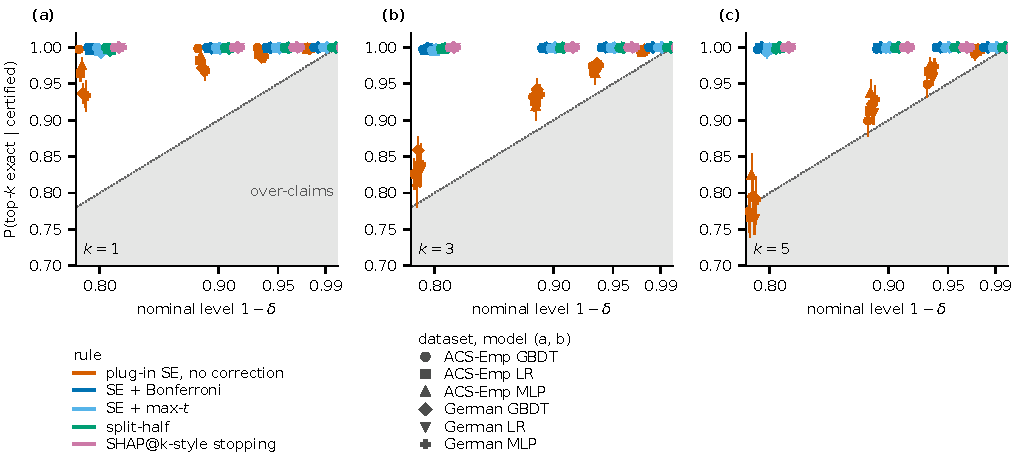
\includegraphics{figA_calibration_k135.pdf}
\caption{Calibration of the certificates for $k=1,3,5$ (as Figure~\ref{fig:cert}a,b).}
\label{fig:cal-k135}
\end{figure}

\begin{figure}[h]
\centering
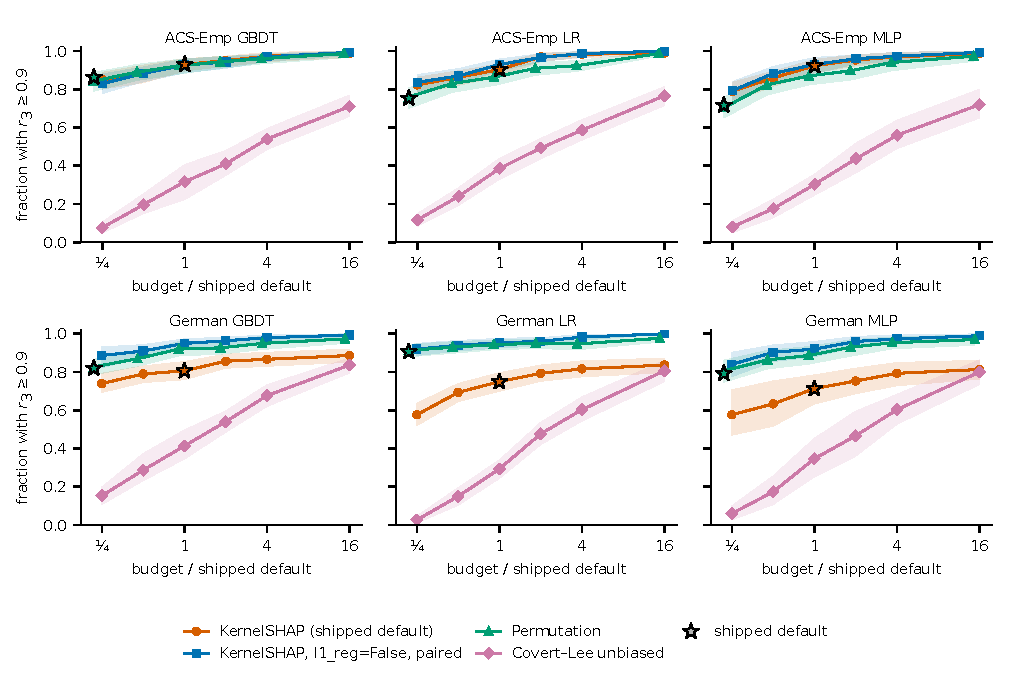
\includegraphics{figA_budget_by_model.pdf}
\caption{As Figure~\ref{fig:budget}, with one panel per dataset and model.}
\label{fig:budget-model}
\end{figure}

\begin{figure}[h]
\centering
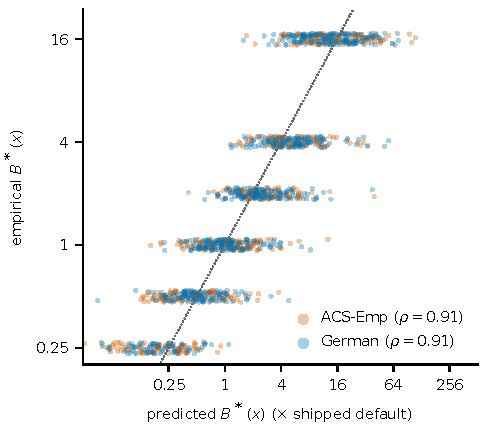
\includegraphics{figA_bstar.pdf}
\caption{Required budget $B^*(x)$ per instance: predicted from $c\sigma^2/\mathrm{gap}^2$ ($c$ fitted per cell) against the smallest grid budget at which $r_3\ge0.9$ (Covert--Lee, $k=3$, $\delta=0.1$). Instances not reliable by $16\times$ are censored there and drawn hollow. Spearman rank correlation over uncensored points in the legend.}
\label{fig:bstar}
\end{figure}

\begin{figure}[h]
\centering
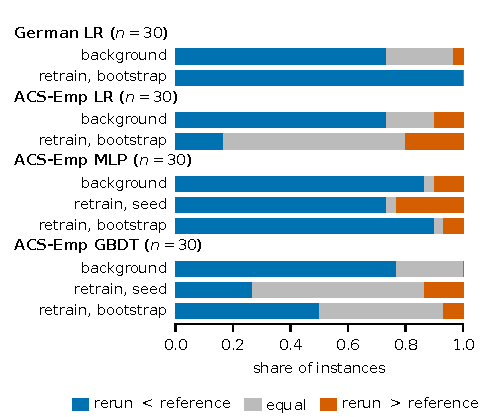
\includegraphics{fig2_yardstick_perm.pdf}
\caption{As Figure~\ref{fig:yardstick}, for the Permutation explainer.}
\label{fig:yardstick-perm}
\end{figure}

\begin{figure}[h]
\centering
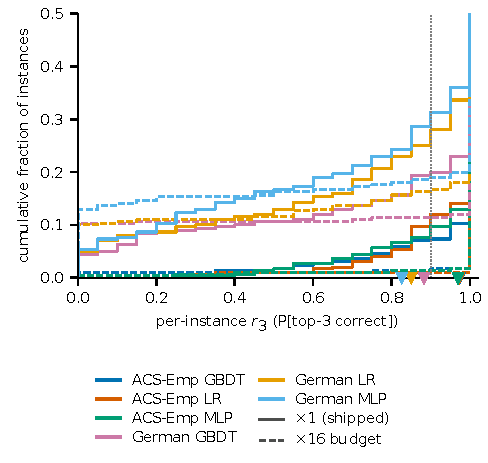
\includegraphics{figA_ecdf_x16.pdf}
\caption{Exact $r_3$ at the shipped budget (solid) and at $16\times$ that budget (dashed), as Figure~\ref{fig:tail}a.}
\label{fig:ecdf16}
\end{figure}

\begin{figure}[h]
\centering
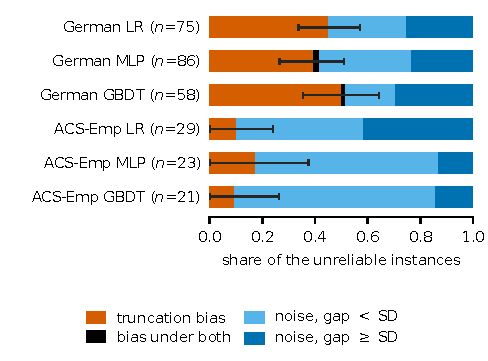
\includegraphics{figA_c5_split.pdf}
\caption{What the unreliable instances of the shipped KernelSHAP default are made of. Per cell group (three seeds pooled), the instances with $r_3<0.9$ at the shipped budget ($n$ in the labels) split by the \emph{mean} attribution of the default's reruns: wrong top-3 under the default but right under paired \texttt{l1\_reg=False} (truncation bias; 95\% cluster-bootstrap interval); wrong under both; right but the runs scatter (noise), split by the gap between the $3$rd and $4$th attribution against the rerun SD of that difference ($z_{\rm true}$ below / at or above 1; a descriptive threshold). Interval widths reflect small $n$ on ACS.}
\label{fig:c5}
\end{figure}

\begin{table}[h]
\caption{Per-cell values behind Table~\ref{tab:cert}.}
\label{tab:cert-cells}
\centering\scriptsize
\begin{tabular}{@{}llccccrr@{}}
\toprule
Dataset, model & Rule & certified & P(exact $\mid$ certified) & delivered correct & coalitions & fixed Covert--Lee & fixed \texttt{l1\_reg=False} \\
\midrule
ACS-Emp GBDT & plug-in SE & 0.78 & 0.932 [0.920, 0.944] & 0.87 & 14148 & 33280 & $\leq$520 \\
 & Bonferroni & 0.50 & 0.999 [0.998, 1.000] & 0.89 & 22955 & n/a & $\leq$520 \\
 & max-$t$ & 0.52 & 0.998 [0.996, 1.000] & 0.89 & 22366 & n/a & $\leq$520 \\
 & split-half & 0.44 & 0.999 [0.997, 1.000] & 0.85 & 25288 & 33280 & $\leq$520 \\
 & SHAP@k & 0.41 & 1.000 [1.000, 1.000] & 0.89 & 25828 & n/a & $\leq$520 \\
\addlinespace[2pt]
ACS-Emp LR & plug-in SE & 0.84 & 0.926 [0.912, 0.937] & 0.89 & 11019 & 33280 & $\leq$520 \\
 & Bonferroni & 0.57 & 0.999 [0.998, 1.000] & 0.92 & 21551 & 33280 & $\leq$520 \\
 & max-$t$ & 0.58 & 0.998 [0.996, 1.000] & 0.92 & 20928 & 33280 & $\leq$520 \\
 & split-half & 0.50 & 0.999 [0.997, 1.000] & 0.88 & 24141 & 33280 & $\leq$520 \\
 & SHAP@k & 0.46 & 1.000 [1.000, 1.000] & 0.92 & 25241 & 33280 & $\leq$520 \\
\addlinespace[2pt]
ACS-Emp MLP & plug-in SE & 0.82 & 0.919 [0.900, 0.937] & 0.87 & 12436 & 33280 & $\leq$520 \\
 & Bonferroni & 0.52 & 0.999 [0.997, 1.000] & 0.90 & 23182 & n/a & $\leq$520 \\
 & max-$t$ & 0.54 & 0.998 [0.996, 1.000] & 0.90 & 22508 & n/a & $\leq$520 \\
 & split-half & 0.44 & 1.000 [1.000, 1.000] & 0.87 & 25703 & 33280 & $\leq$520 \\
 & SHAP@k & 0.40 & 1.000 [1.000, 1.000] & 0.90 & 26685 & n/a & $\leq$520 \\
\addlinespace[2pt]
German GBDT & plug-in SE & 0.88 & 0.942 [0.927, 0.957] & 0.91 & 9647 & 33408 & $\leq$522 \\
 & Bonferroni & 0.62 & 0.999 [0.998, 1.000] & 0.94 & 20218 & 33408 & $\leq$522 \\
 & max-$t$ & 0.64 & 0.999 [0.998, 1.000] & 0.94 & 19561 & 33408 & $\leq$522 \\
 & split-half & 0.54 & 0.999 [0.997, 1.000] & 0.91 & 22919 & 33408 & $\leq$522 \\
 & SHAP@k & 0.49 & 1.000 [1.000, 1.000] & 0.94 & 24092 & 33408 & $\leq$522 \\
\addlinespace[2pt]
German LR & plug-in SE & 0.85 & 0.933 [0.918, 0.945] & 0.90 & 12136 & 33408 & $\leq$522 \\
 & Bonferroni & 0.55 & 0.999 [0.998, 1.000] & 0.92 & 23782 & 33408 & $\leq$522 \\
 & max-$t$ & 0.57 & 0.999 [0.998, 1.000] & 0.92 & 23097 & 33408 & $\leq$522 \\
 & split-half & 0.45 & 1.000 [1.000, 1.000] & 0.90 & 26943 & 33408 & $\leq$522 \\
 & SHAP@k & 0.40 & 1.000 [1.000, 1.000] & 0.92 & 28187 & 33408 & $\leq$522 \\
\addlinespace[2pt]
German MLP & plug-in SE & 0.83 & 0.935 [0.918, 0.949] & 0.89 & 12118 & 33408 & $\leq$522 \\
 & Bonferroni & 0.56 & 0.999 [0.998, 1.000] & 0.92 & 22969 & 33408 & $\leq$522 \\
 & max-$t$ & 0.58 & 0.999 [0.998, 1.000] & 0.92 & 22348 & 33408 & $\leq$522 \\
 & split-half & 0.47 & 1.000 [1.000, 1.000] & 0.89 & 26039 & 33408 & $\leq$522 \\
 & SHAP@k & 0.42 & 1.000 [1.000, 1.000] & 0.92 & 27280 & 33408 & $\leq$522 \\
\bottomrule
\end{tabular}

\end{table}
